%! TeX Program = LuaLaTeX
\documentclass[twoside]{article}
\usepackage[margin=1.2in]{geometry}
\usepackage{graphicx}
\usepackage{fontspec, luatexja}
\newfontfeature{microtype}{protrusion=default;expansion=default}
\defaultfontfeatures{microtype}
\adjustspacing=2
\protrudechars=2
\setmainfont{Linux Libertine O}
\setsansfont{Linux Biolinum O}
\setmonofont[Scale = MatchLowercase, FakeStretch = 1.137121]{Iosevka Slab}
\usepackage{listings}
\lstset{
    basicstyle = \ttfamily\small,
    breaklines = true,
    columns = fullflexible,
    keepspaces = true,
    numbers = left,
    numberstyle = \tiny,
    stepnumber = 1,
    gobble = 4,
    numbersep = 6pt,
    escapechar = §
}
\usepackage{hyperref}
\hypersetup{
    hidelinks,
    pdftitle = {Evangelion-JFM},
    pdfauthor = {Jing Huang},
    pdfsubject = {TeX},
    pdfkeywords = {Japanese Font Metric},
    pdfstartview = FitV
}
\long\def\feature#1#2#3{{\vskip8pt\vbox{\normalsize\parindent=\zw\hangindent=2\zw\rightskip=2\zw\texttt{#1 --> ({\itshape #2\/})}\\\indent#3\par}}}
\def\meta#1{{\normalfont\rmfamily\itshape$\langle$#1\/$\rangle$}}
\def\LuaTeX{Lua\kern-.2ex\TeX}
\def\pTeX{p\kern-.2ex\TeX}
\def\pdfTeX{pdf\TeX}
\title{\sffamily\bfseries Evangelion Japanese Font Metric for \LuaTeX}
\author{\large \url{https://github.com/RadioNoiseE/Evangelion-JFM}\\\url{https://www.ctan.org/pkg/evangelion-jfm}}
\date{2023, Jing Huang (黄京)}
\begin{document}
\parindent=12pt\parskip=2pt
\maketitle

\begin{abstract}
    This documentation is going to introduce Evangelion Japanese Font Metric (hereinafter referred to as ``\textsf{Eva-JFM}''), a Japanese Font Metric for typesetting high quality Chinese and Japanese documents. It can be used with Traditional Chinese, Simplified Chinese and Japanese fonts for both vertically and horizontally typesetted texts. It aims to provide a font metric which makes full use of the \texttt{priority} feature (provided by \textsf{\LuaTeX-ja}), bases on the standard~\cite{jlreq}, and supports some advanced (a.k.a., rarely-used) features. The documentation is now written in Chinese, Japanese and English.\par
    This documentation is far from complete. It may have many grammatical (and contextual) errors.
\end{abstract}

\tableofcontents

\section{Background Information and a Rough Introduction}
{\TeX} is a powerful typesetting system ``intended for the creation of beautiful books'', it has full support for typesetting English based texts. However, its support for CJ text is limited\footnote{Maybe because there was no universally recognized or accepted CJ character set standard as well as an encoding system.}. For handling CJ texts in {\TeX}, both macro extensions (i.e., \textsf{CJK}) and engine extensions were developed. One of the most influential one is (the) {\pTeX} (series).\par
{\pTeX} uses a virtual font scheme, by mapping TrueType or OpenType fonts using \texttt{TFM/VF} files. It doesn't support font configuration through macros, and has no support for PDF format output. Its advantage is the proven ability for dealing with traditional Japanese typographic layout requirements.\par
{\pdfTeX} is a {\TeX} engine extension which can directly output PDF files (just as its name). But it has limited support to Unicode as well as modern font formats (TrueType and OpenType vector font formats).\par
{\LuaTeX} is based on {\pdfTeX}. The inclusion of Lua enables it to support Unicode with the \textsf{reader} module, and modern fonts by using \textsf{fontloader}. Its macro based font setup feature is provided by \textsf{luaotfload}.\par
\LuaTeX-ja can be seen as a porting of {\pTeX} and {\LuaTeX}. It's a macro package for typesetting high quality Japanese documents when using {\LuaTeX}. {\LuaTeX} supports font configuring by macros, therefore there's no need to keep {\pTeX}'s \texttt{VF} file. But for advanced features it left and extended\footnote{The \texttt{priority} feature and some imaginary characters as well.} the so-called JFM file.\par
This document describes \textsf{Eva-JFM}, an advanced JFM file. By using {\LuaTeX}'s callback, it embeds features (maybe) needed in CJ text typesetting in \texttt{Eva-JFM.lua}. The features supported now are ``Traditional Chinese'', ``Simplified Chinese'', ``Japanese'', ``Vertical Typesetting'', ``Linegap Punctuations'', ``Hanging Punctuations'', ``Extended Font'', and ``Non Standard''.

\section{Installation and Local Configurations}
The sourcefiles are hosted on Github while it's also uploaded to CTAN. Users can simply use
\begin{lstlisting}
    tlmgr install evangelion-jfm
\end{lstlisting}
(or maybe using other package managers) to install. (But note that the CTAN branch is not always updated.) Developers can also use
\begin{lstlisting}
    mkdir Evangelion-JFM [&&] cd Evangelion-JFM
    git clone https://github.com/RadioNoiseE/Evangelion-JFM
\end{lstlisting}
to extract the latest version, then move it to the \texttt{TEXMF} directory, for instance
\begin{lstlisting}
    ~/Library/texlive/2023/texmf-dist/tex/luatex/eva-jfm
\end{lstlisting}
If your {\TeX} distribution requires
\begin{lstlisting}
    mktexlsr
\end{lstlisting}
to update the \texttt{Ls-R} database, make it so.\par
\textsf{Eva-JFM} doesn't require any local configuration in most cases, but if you have some special requirements, have a look at section \ref{sec:config}.

\section{Using}
The above is an example of typesetting vertical text using Traditional Chinese fonts
\begin{lstlisting}
    \usepackage{luatexja-fontspec, luatexja-adjust}
    \setmainjfont{Source Han Serif TC}[Language = Chinese Traditional, TateFeatures = {JFM = eva/{vert, trad, nstd}}]
    \ltjenableadjust[priority = true]
\end{lstlisting}
(and be aware that you need to load a document class which supports vertical typesetting or use the \texttt{\string\tate} command. \LuaTeX-ja's JFM syntax is the above
\begin{lstlisting}
    jfm = §\meta{JFM name}§/{§\meta{JFM features}§}
\end{lstlisting}
while under {\LaTeX} the most common case while using \texttt{\string\setmainjfont} is most likely
\begin{lstlisting}
    \setmainjfont{§\meta{font name}§}[Language = §\meta{language name}§, §\meta{dir}§ = {JFM = §\meta{JFM name}§/{§\meta{JFM features}§}}]
\end{lstlisting}
Option \meta{font name} is the font (that you'd like to specify as the main font for your document)'s name. When using Japanese fonts, simply ignore the \meta{language name} since \LuaTeX-ja will automatically fill it for you. In this case, filling \texttt{Chinese} \texttt{Traditional} for Traditional Chinese fonts and \texttt{Chinese} \texttt{Simplified} for Simplified Chinese fonts is necessary\footnote{Without this, your output may result in wrong details, for instance wrong punctuation shape \& direction.}. \meta{dir} should be \texttt{TateFeatures} when typeset vertically and \texttt{YokoFeatures} for typesetting horizontally accordingly. The JFM's name is specified by the \meta{JFM name} option\footnote{\LuaTeX-ja searchs for a JFM file following the method \texttt{jfm-\meta{JFM name}.lua}.}. Finally, for the \meta{JFM features} key, fill in the JFM features. They are described in section \ref{sec:feat}.\par
For advanced users, it's also recommanded to use the following
\begin{lstlisting}
    \def\ltj@stdyokojfm{eva/{§\meta{JFM features}§}}
\end{lstlisting}
or with the NFSS.\par
To set up JFM in other cases, please refer to the \LuaTeX-ja document~\cite{luatexja-doc}.

\section{Supported Features}
\label{sec:feat}
This section is going to give you a glance at all the features embedded in \textsf{Eva-JFM}. They are divided into 5 groups, and are described in the next 5 subsections respectively.

\subsection{Language Features}
You should specify one and only one feature from this section, or your {\TeX} is going to complain about it.\par
\feature{jp}{JaPanese}{%
    Japanese font feature. When using Japanese fonts, you are required to specify this. It's very difference from Traditional Chinese and Simplified Chinese feature, namely the glue inserted after Question Mark and Exclamation Mark, and some punctuation mark's position when typeset vertically. It affects the feature \texttt{lgp}, as well as the internal grouping.\par
}
\feature{trad}{TRADitional chinese}{%
    Traditional Chinese feature. You should specify this when you are typesetting using Traditional Chinese fonts. The differences from the other two is because of its middle-placed punctuations. Hence the glues inserted next to it, the line-end adjust, as well as some kernings between punctuations are special.
}
\feature{smpl}{SiMPLified chinese}{%
    Simplified Chinese feature, for Simplified Chinese fonts. Almost all the punctuations are laid down and placed aside. Therefore its position is treated with care. \textsf{Eva-JFM} also takes some rare conditions into consideration. Note that the \textit{aki\/} after Question Mark and Exclamation Mark is different from that of the Japanese font feature.
}

\subsection{Direction Features}
Features in this section is compatible with all the other features.\par
\feature{vert}{VERTical writing}{%
    Vertical Typesetting feature. It affects kerning, internal grouping, etc. You should specify this when typeseting vertically.
}

\subsection{Extended Features}
Except the feature \texttt{hgp} doesn't rely on feature \texttt{vert}, all the other features need \texttt{vert} to work (since they should only be needed in vertical texts).
\feature{extd}{EXTenDed font}{%
    Extended font features. The dafault ratio is \textit{x\/}:\textit{y\/}=100:80 while \textit{x\/} is the width and \textit{y\/} is the height. You can customize it using \texttt{extd=\meta{ratio}} (the dafault \meta{ratio} is 1.25). It should be used with \texttt{extend} (\textsf{luaotfload}) or \texttt{FakeStretch} (\textsf{fontspec}).
}
\feature{lgp}{LineGap Punctuations}{%
    The linegap punctuations feature. This hangs some punctuations into the linegap. Some difference occurs when it's used with the \texttt{jp} feature. For more information see section~\ref{sec:lgp}.
}
\feature{hgp}{HanGing Punctuations}{%
    Hanging punctuation feature which ``hangs'' some punctuation at line-end (allowing them to stick out a bit). Traditional Chinese fonts doesn't support this feature because the result is somewhat (rather) wierd.
}

\subsection{English Features}
You need to set the JAchar range using \texttt{\string\ltjsetparameter} before using features in this section, or they won't work properly. It's also recommended to use with the corresponding OpenType features.\par
\feature{hwid}{Half WIDth}{%
    Half width English characters feature. This will place each alphabets into a box which width is exactly 0.5 times the CJ character's width. It's worth noting that it will not stretch or shrink the glyph, it only adjusts the spacing. Hence if the OpenType feature \texttt{hwid} is not set, English characters will simply overlap. All the kernings and italic corrections will also be lost (this may be fixed in the future versions), and will ignore the parameter \texttt{xkanjiskip}. Please use with care.
}
\feature{fwid}{Full WIDth}{%
    Full width English characters feature. It's similar from feature \texttt{hwid} above except that the spacing will be stretched out on the contrary.
}

\subsection{Dark Features}
Before using the following features, please make sure that you have carefully read the descriptions.\par
\feature{nstd}{Non STandarD}{%
    This one ignores the standard priority rules for punctuation kerning. While Japanese text layout requirement~\cite{jlreq} suggests that the priority for the period should be higher than the comma (which means the period is easier to stretch), this makes the comma's priority higher than the preiod's. Only works when \textsf{luatexja-adjust}'s priority feature is enabled (set to \texttt{true}).
}
\feature{plain}{PLAIN punct kerning style}{%
    Disables the performance of spaceing adjustment for any of the puncts. Designed to be used in the verbatim environment. Developers can use the hook provided by that environment to specify this feature.
}

\section{Linegap Punctuation Feature}
\label{sec:lgp}
Here more detailed information about linegap punctuations are provided, as well as the issues may occur and the possible solution.
\subsection{About ``Hanging''}
Linegap punctuations can be seen in Chinese ancient books, it's a combination of the punctuations marks and the traditional vertical typesetting method.\par
Only periods and commas should be hanged but \textsf{Eva-JFM} hangs three more punctuations in addition. Japanese font is different in this aspect however, since the direction of colon and semicolon makes it impossible to be hanged.\par
They are all hanged to the lower right of the glyph. See the next subsection for more details.

\subsection{Hanging Position}
\begin{figure}[htb]
    \centering
    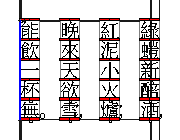
\includegraphics[height = 120pt]{figure/fig-tc.pdf}\quad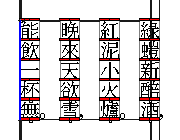
\includegraphics[height = 120pt]{figure/fig-jp.pdf}
    \caption{The linegap punctuations feature}
    \label{fig:lgp}
\end{figure}
The position of these hanged punctuations is decided according to the following rules as shown in the figure \ref{fig:lgp}. For customizing, see subsection~\ref{sec:config}. The rules which occurs more early have the higher priorities.
\begin{itemize}
    \item The style of the three fonts are unified;
    \item The position of the similar elements in different punctuations should be the same;
    \item The glyph of the punctuations should touch the \textit{kanji\/}'s boundary;
    \item Different punctuations' position can vary considering their glyphs' shapes, sizes, design respectively.
\end{itemize}

\subsection{User Configs}
\label{sec:config}
This feature is designed for the Source Han font series (思源系列). Due to different fonts' different punctuation marks, the output may be wrong (overlap, not aligned, etc). Also you may prefer your own settings. Therefore, two methods of customizing the positions of hanged punctuations is provided here.

\subsubsection{Changing Parameters}
In \textsf{Eva-JFM}, the tables which contains the parameters for the positions of these hanged punctuations is
\begin{lstlisting}
    [101,2] ==> [1]; [201,2] ==> [2]; [301,2] ==> [3].
\end{lstlisting}
Kindly modify \texttt{left} (dir right) and \texttt{down} (dir down) until the output is fine.
You can also refer to the last section (\textit{Implementing\/}).

\subsubsection{Using Extra Font}
Extracting the glyphs for punctuation marks and package them into a new font (you can use programs like \textit{fontforge\/}) and use them for hanging punctuations later is the second solution. You can also load another font just for its punctuations (but loading a CJ font into {\TeX}'s memory has an expensive cost).\par
After installing that font, you can use the \texttt{AltFont} key provided by \LuaTeX-ja to replace the punctuations. The actual code is shown above.
\begin{lstlisting}
    \setmainjfont[
        Language = §\meta{language}§,
        TateFeatures = {
            JFM = eva/{vert, lgp, §\meta{language}§},
            AltFont = {
                {Range = "§\meta{utf-8 code}§, Font = §\meta{symbol font}§}
            }
        }
    ]{§\meta{main font}§}
\end{lstlisting}
One of \texttt{Japanese}, \texttt{Chinese} \texttt{Traditional} or \texttt{Chinese} \texttt{Simplified} should be filled in the first \meta{language} option, the other one is for the corresponding JFM features. \meta{utf-8 code} selects the punctuations you'd like to replace with the ``punctuation font''\footnote{You can search \url{https://www.unicode.org/charts/unihanrsindex.html} for their unicodes representations.}.
Finally, it's obvious that the \meta{symbol font} and the \meta{main font} options are for the ``punctuation font'' and the main font.\par
It's also recommended for the developers to use the NFSS with
\begin{lstlisting}
    \DeclareAlternateKanjiFont{§\meta{base encoding}§}{§\meta{base family}§}{§\meta{base series}§}{§\meta{base shape}§}{§\meta{alt encoding}§}{§\meta{alt family}§}{§\meta{alt series}§}{§\meta{alt shape}§}{§\meta{range}§}
\end{lstlisting}
Option \meta{base} and \meta{alt} stands for main font and ``punctuation font''.\par
Refer to the \LuaTeX-ja document~\cite{luatexja-doc} for more detailed syntax and usage as well as some examples.

\section{Inspiration}
\textsf{Eva-JFM}'s internal grouping is inspired by \texttt{min10.tfm}~\cite{min10}, while its \texttt{priority} feature's data partly comes from Noriyuki Abe's \texttt{jlreq.lua}~\cite{ltxjlreq}.\par
This JFM's name comes from the animation \textit{Neon Genesis Evangelion\/} by Hideaki Anno.

\begin{thebibliography}{9}
    \addcontentsline{toc}{section}{\refname}
    \bibitem{jlreq} W3C Japanese Layout Task Force~(ed). \newblock Requirements for Japanese Text Layout (W3C Working Group Note), 2022, 2023. \newblock \url{https://www.w3.org/TR/jlreq/}.
    \bibitem{luatexja-doc} \LuaTeX-jaプロジェクトチーム. \newblock \LuaTeX-jaパッケージ, 2022, 2023.
    \bibitem{unicode} The Unicode Consortium. \newblock The Unicode Standard Version 15.0 - Core Specification, 2022.
    \bibitem{tex-by-topic} Victor Eijkhout. \newblock \TeX{} by Topic, A \TeX nician's Reference, Addison-Wesley, 1992.
    \bibitem{min10} 乙部厳己. \newblock min10フォントについて. \newblock \url{http://argent.shinshu-u.ac.jp/~otobe/tex/files/min10.pdf}.
    \bibitem{ltxjlreq} 阿部紀行. \newblock Jlreq Document Class, 2022. \newblock \url{https://github.com/abenori/jlreq}.
    \bibitem{evang} 庵野秀明. \newblock 新世紀エヴァンゲリオン.
\end{thebibliography}


\end{document}
